% -*- compile-command: "latexmk -pdf document.tex" -*-
\documentclass{article}

\author{Sam Price}
\title{Cantor Set}

\newif\ifprinted%
\printedtrue%
% Most taken from: https://github.com/SeniorMars/dotfiles/blob/main/latex_template/preamble.tex
\usepackage{geometry}

\usepackage[english]{babel}
\usepackage[T1]{fontenc}
\usepackage[utf8]{inputenc}
\usepackage{palatino}

% Use the command \doublespacing if needed
\usepackage{setspace}

\geometry{a4paper, margin=1in}

\usepackage{mathtools}
\usepackage{amssymb,amsfonts,amsthm,amsmath}

\usepackage{xfrac}
\usepackage[makeroom]{cancel}

% Use \begin{enumerate}[start=x,label={Q\arabic*)}] for example
\usepackage{enumitem}

\usepackage{xcolor}

\usepackage{nameref}

% Important options
% in envs, use options like [baseline=x] to center on row x (or special opts t/[c]/b without 'baseline')
\usepackage{nicematrix}
\NiceMatrixOptions{cell-space-limits = 1pt}

\usepackage{booktabs}

\usepackage{tikz}
\usepackage{tikz-cd}
\usepackage{tikzsymbols}

\usepackage{pdfpages}

\usepackage[most,many,breakable]{tcolorbox}

\setlength{\parindent}{1cm}

\DeclarePairedDelimiter{\abs}{\lvert}{\rvert}

%%%%%%%%%%%%%%%%%%%%%
%%% THEOREM BOXES %%%
%%%%%%%%%%%%%%%%%%%%%
\definecolor{thmbgcol}{HTML}{aec1f9}
\definecolor{thmhlcol}{HTML}{142c72}
\definecolor{corbgcol}{HTML}{b599f7}
\definecolor{corhlcol}{HTML}{2d1760}
\definecolor{propbgcol}{HTML}{c9f7aa}
\definecolor{prophlcol}{HTML}{1e631a}
\definecolor{exbgcol}{HTML}{f7c479}
\definecolor{exhlcol}{HTML}{604419}

\definecolor{qheadcol}{HTML}{182959}

\tcbuselibrary{theorems,skins,hooks}
\newtcbtheorem[number within = section]{theorem}{Theorem}{
  enhanced, breakable, colback = thmbgcol!25,
  frame hidden, boxrule = 0sp, borderline west = {2pt}{0pt}{thmhlcol},
  sharp corners, detach title, before upper = \tcbtitle\par\smallskip,
  coltitle = thmhlcol, fonttitle = \bfseries,
  description font = \mdseries, separator sign none, segmentation style = {solid, thmhlcol}
}{th}

\newtcbtheorem[number within = section]{corollary}{Corollary}{
  enhanced, breakable, colback = corbgcol!25,
  frame hidden, boxrule = 0sp, borderline west = {2pt}{0pt}{corhlcol},
  sharp corners, detach title, before upper = \tcbtitle\par\smallskip,
  coltitle = corhlcol, fonttitle = \bfseries,
  description font = \mdseries, separator sign none, segmentation style = {solid, corhlcol}
}{cor}

\newtcbtheorem[number within = section]{proposition}{Proposition}{
  enhanced, breakable, colback = propbgcol!25,
  frame hidden, boxrule = 0sp, borderline west = {2pt}{0pt}{prophlcol},
  sharp corners, detach title, before upper = \tcbtitle\par\smallskip,
  coltitle = prophlcol, fonttitle = \bfseries,
  description font = \mdseries, separator sign none, segmentation style = {solid, prophlcol}
}{prop}

\newtcbtheorem[number within = section]{example}{Example}{
  enhanced, breakable, colback = exbgcol!25,
  frame hidden, boxrule = 0sp, borderline west = {2pt}{0pt}{exhlcol},
  sharp corners, detach title, before upper = \tcbtitle\par\smallskip,
  coltitle = exhlcol, fonttitle = \bfseries,
  description font = \mdseries, separator sign none, segmentation style = {solid, exhlcol}
}{prop}

\newtcbtheorem[number within = section]{definition}{Definition}{
  enhanced, breakable, colback = red!10,
  frame hidden, boxrule = 0sp, borderline west = {2pt}{0pt}{red!50!black},
  sharp corners, detach title, before upper = \tcbtitle\par\smallskip,
  coltitle = red!50!black, fonttitle = \bfseries,
  description font = \mdseries, separator sign none, segmentation style = {solid, exhlcol}
}{def}

\makeatletter
\newtcbtheorem{question}{Question}{enhanced,
    breakable,
    colback=white,
    colframe=qheadcol,
    attach boxed title to top left={yshift*=-\tcboxedtitleheight},
    fonttitle=\bfseries,
    title={#2},
    boxed title size=title,
    boxed title style={%
            sharp corners,
            rounded corners=northwest,
            colback=qheadcol,
            boxrule=0pt,
        },
    underlay boxed title={%
            \path[fill=tcbcolframe] (title.south west)--(title.south east)
            to[out=0, in=180] ([xshift=5mm]title.east)--
            (title.center-|frame.east)
            [rounded corners=\kvtcb@arc] |-
            (frame.north) -| cycle;
        },
    #1
}{def}
\makeatother


\newcommand{\CA}{\mathcal{C}}

\begin{document}

\maketitle

Let $C_{0} = [0, 1]$, and define a sequence of sets by
\[ C_{n + 1} = \frac{1}{3}C_{n} \cup \frac{2}{3} + \frac{1}{3}C_{n}. \]
That is, remove the middle third of every closed interval each iteration.
Call $\CA = C_{\infty}$ or equivalently $\cap C_{i}$ for all $i \in \NN$.

\begin{enumerate}[start=1,label={\arabic*\rparen}]
  \item Sketch $C_{n}$ for $n \le 4$. (Picture hopefully included, I decided to write out intervals for $C_{4}$ because OH MY)
  \item Show $\CA$ is uncountable.
  \item Show $\CA$ has measure zero.
\end{enumerate}

For the first, here's the picture:

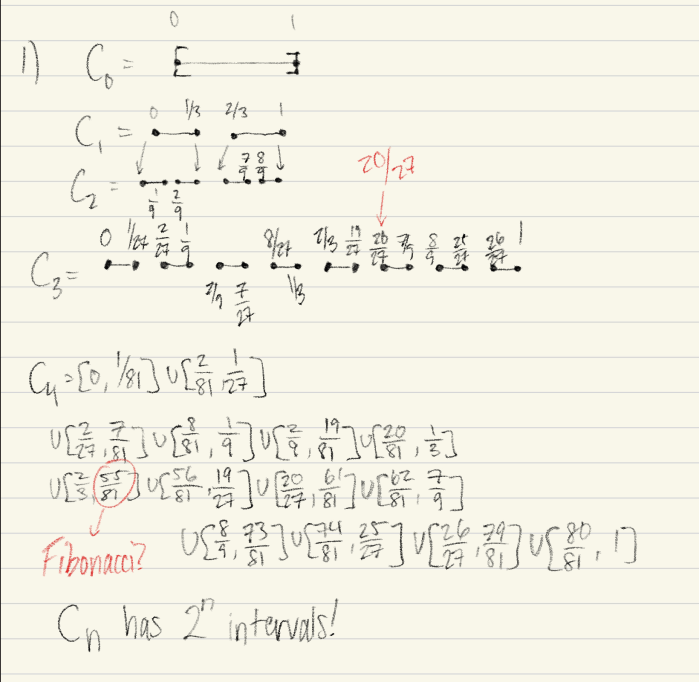
\includegraphics[width=\textwidth/2]{cantor}

For the second, suppose that $\CA = \set{ a_{1}, \ldots }$ and is countable.
Then, $a_{1} \in C_{1}$
\footnote{or go until we do have one such $a_{k}$, but we assume throughout we can always find the ``next'' one where desired}
and so either $a_{1} \in [0, 1/3]$ or $a_{1} \in [2/3, 1]$.
Choose the interval $a_{1}$ is \textbf{not} included within, and call it $I_{1}$.
Then, $a_{2} \in I_{1}$ and so without loss of generality
either $a_{2} \in [0,1/9]$ or $a_{2} \in [2/9, 1/3]$.
Again, call the interval it is \textbf{not} within $I_{2}$.
We then have a sequence
\[ I_{1} \supset I_{2} \supset \cdots \]
where $a_{k} \notin I_{k}$.
However, there must still be some $x \in \cap I_{n}$ since it is the intersection of nested closed
intervals\footnote{Failed to prove this in 301} that \emph{isn't} inside of $\CA$ which is
obviously contradictory. So, $\CA$ is uncountable.

Finally we want to show that $\CA$ has measure zero.
Let us first consider the sequence of measures of the $C_{n}$ in our construction:
\[
  \set{ m(C_{0}), m(C_{1}), m(C_{2}), \ldots }
  =
  \set{ 1, 2/3, 4/9, \ldots }.
\]
By being careful, we can see that $C_{k}$ has measure $\pars{2/3}^{k}$.
Since $\CA$ is the \emph{intersection} of all these sets, it cannot have a measure
greater than the infimum of this sequence. However, $\pars{2/3}^{k} \to 0$ as $k \to \infty$
and so $\CA$ has to have zero measure exactly.

\end{document}
